%%%%%%%%%%%%%%%%%%%%%%%%%%%%%%%%%%%%%%%%%%%%%%%%%%%%%%%%%%%%%%%%%%%%%
% Imperial College
\documentclass[a4paper,11pt,twoside]{article}
\usepackage[left=2.5cm,right=2cm,top=2cm,bottom=2cm]{geometry}

%%%%%%%%%%%%%%%%%%%%%%%%%%%%%%%%%%%%%%%%%%%%%%%%%%%%%%%%%%%%%%%%%%%%%
% Paragraph
\usepackage[parfill]{parskip}

% Images
\usepackage{graphicx}

% URLs
\usepackage{hyperref}

% Maths
\usepackage{amsmath}

%%%%%%%%%%%%%%%%%%%%%%%%%%%%%%%%%%%%%%%%%%%%%%%%%%%%%%%%%%%%%%%%%%%%%
\begin{document}
\title{Testing Numerical Methods for Integrating Systems of ODEs using 
the Case of a Pendulum}
\author{Dakshina Scott}
\date{\today}
\maketitle

%%%%%%%%%%%%%%%%%%%%%%%%%%%%%%%%%%%%%%%%%%%%%%%%%%%%%%%%%%%%%%%%%%%%%
\begin{abstract}

\end{abstract}

%%%%%%%%%%%%%%%%%%%%%%%%%%%%%%%%%%%%%%%%%%%%%%%%%%%%%%%%%%%%%%%%%%%%%

\tableofcontents

%%%%%%%%%%%%%%%%%%%%%%%%%%%%%%%%%%%%%%%%%%%%%%%%%%%%%%%%%%%%%%%%%%%%%

\section{Introduction}
In this investigation we begin by using the dynamics of a simple 
pendulum to examine three methods of numerical integration - Euler's
method, the leapfrog method, and the fourth-order Runge-Kutta 
method(RK4). Based on stability analyses of each method the most 
appropriate one is then chosen for use on a double pendulum. Due to the 
chaotic nature of a double pendulum system it is important that 
the chosen method is the most stable/accurate???. 

\section{Euler's Method}
Euler's method is the most simple method for numerically integrating a 
system of ODEs with given initial conditions. In this method the value 
of the derivative at an initial point is used to estimate a new value 
after a small step forward in the x-axis. This apprach works well on
functions with constant or slowly changing gradients, but for a 
a function with a rapidly changing gradient (e.g. oscilating) one would 
not expect this to give very good estimates.

\begin{figure}{htb}
	\centering
	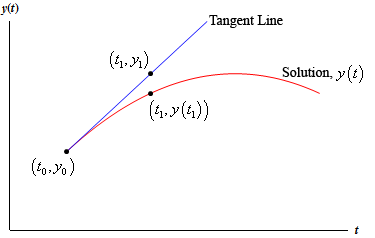
\includegraphics[width=0.8\textwidth]{euler_example.png}
	\caption{}
	\label{fig:euler_example}
\end{figure}
 
%%%%%%%%%%%%%%%%%%%%%%%%%%%%%%%%%%%%%%%%%%%%%%%%%%%%%%%%%%%%%%%%%%%%%
\begin{thebibliography}{20}

bibitem{euler_example}
Paul's Online Math Notes, 2012. [online] Available at \url{http://tutorial.math.lamar.edu/Classes/DE/EulersMethod.asp}
[Accessed 8 November 2012].

\end{thebibliography}

\end{document}

